\documentclass[main.tex]{subfiles}

\begin{document}
    \chapter{Introduction}
    \setlength{\epigraphwidth}{0.8\textwidth}
    % \epigraph{
    %         \selectlanguage{greek}
    %         >en p~asi g`ar to~is fusiko~is >'enest'i ti jaumast'on\\
    %         \vspace{0.2cm}
    %         \selectlanguage{english}
    %         In all things of nature there is something of the marvelous
    % }{--- Aristotle, 384-322 BC}
        \epigraph{
            \selectlanguage{english}
            ``You must have chaos within you to give birth to a dancing star''
    }{--- Friedrich Nietzsche, Thus Spoke Zarathustra}
    % \vspace{2cm}

    % Stellar astrophysics has enjoyed remarkable progress over the years, fueled by a synergy between human curiosity and technological innovation.
    From the early days when astronomers gazed at the night sky to the present era of cutting-edge instruments and sophisticated computational models, our comprehension of the structure and evolution of stars has grown exponentially. Although many fundamental processes are still poorly understood (e.g., the theory of convection and internal mixing, the effects of rotation and magnetic fields), improvements in both the quantity and quality of observational data, coupled with significant progress in theoretical advancements and the adoption of novel computational techniques, have allowed for an enormous expansion and refinement of both the formal and conceptual basis of the subject.

    
    % In this introductory chapter, we embark on an exploration of the foundations of stellar astrophysics, tracing the evolution of stars from their birth to their final stages as compact stellar remnants.
    % Amidst this cosmic journey, however, few entities encapsulate the essence of cosmic endurance as profoundly as neutron stars. Forged in the cataclysmic furnace of a dying star, these enigmatic remnants stand as extraordinary celestial laboratories, offering profound insights into the fundamental nature of matter and the extremes of gravity. This dissertation aims to contribute to our understanding of the structure and mass distribution of neutron stars by unraveling the nuanced processes governing the life cycles of these remarkable objects.
    In this introductory chapter, we investigate the fundamentals of stellar astrophysics, examining how stars evolve from their formation to their eventual transformation into compact stellar remnants. During this exploration, we focus particularly on neutron stars, which hold significant importance in astrophysics. Formed from the remnants of dying stars, neutron stars serve as unique celestial laboratories, providing valuable insights into the nature of matter and the effects of strong gravity. This dissertation aims to contribute to our understanding of neutron stars by investigating the intricate processes that govern their life cycles, with a specific emphasis on their structure and mass distribution.

    Naturally, it has been necessary to be selective in the material presented. The intention here is to lay the groundwork and provide a succinct overview of key concepts tailored to the dissertation's scope, steering away from an exhaustive exploration of stellar astrophysics principles. However, readers seeking further clarification may find additional resources in classical textbooks that offer extensive coverage across diverse facets of this field \citep[e.g.,][]{Clayton, Prialnik, Eggleton, Kippenhahn, Carroll_Ostlie_2017}.

    
    {\hypersetup{linkcolor=black, pdfborder=0 0 1}
    \adjustmtc
    \adjustmtc
    \minitoc
    \newpage
    }
    
    
    
    \section{A Brief Introduction to Stellar Structure \& Evolution}
    From humanity's standpoint, stars often appear as timeless entities, seemingly having existed for eternity and destined to persist indefinitely in the vast expanse of the Universe. This perception, however, is an illusion, stemming from the limited time span during which we observe these celestial bodies in relation to their overall lifetime. In reality, stars undergo the complex processes of birth, evolution, and eventual demise within the cosmic landscape, unfolding over timescales beyond human intuition. To comprehend the evolution of stars over time, observational studies inherently rely on short-term measurements taken from extensive populations.
    Consider the analogy of a paleoanthropologist studying the biological and cultural evolution of humans throughout history. With the first appearance of Homo sapiens believed to have occurred approximately \SI{200000}{years} ago, the only viable method for such a study is through the examination of a large population of fossil records and archaeological evidence spanning different evolutionary stages.

    Given a large sample of stars, we may construct the so-called \textit{``Hertzsprung-Russell diagram''} (H-R diagram), where stars' luminosity is plotted against their effective surface temperature\footnote{It is worth noting that variations of the H-R diagram exist. In alternative forms, the diagram may employ color, magnitude, or spectral type on its axes. For instance, a Color-Magnitude Diagram (CMD) is a variation that plots stars based on their color and magnitude, providing insights into stellar populations and evolutionary stages based on these observable characteristics.}, an example of which can be seen in Fig.~\ref{fig:hrd_gaia}. This diagram provides a visual representation of stellar characteristics, allowing us to organize and analyze large populations of stars simultaneously. Through the H-R diagram, stars can be classified based on their luminosity, temperature, and evolutionary stage, providing a comprehensive snapshot of various stellar life cycles. Much like the paleoanthropologist's careful examination of diverse fossil records, the H-R diagram offers astronomers a panoramic view of stellar evolution, enabling them to unravel the mysteries embedded in stellar dynamics.

    \begin{figure}[h!]
        \centering
        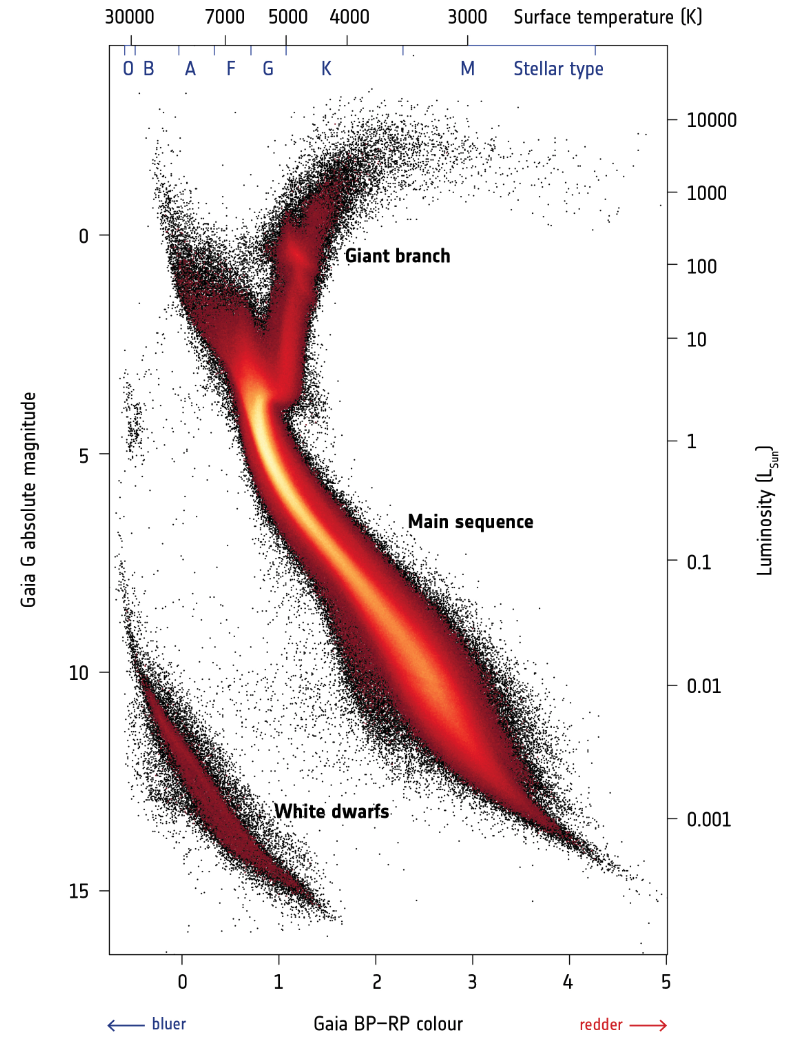
\includegraphics[scale=0.25]{figures/chapter1/hrd_gaia.png}
        \caption{Hertzsprung-Russell diagram obtained by a selection of stars from the second release catalogue of ESA's Gaia satellite. Copyright: \href{https://sci.esa.int/web/gaia/-/60198-gaia-hertzsprung-russell-diagram}{ESA/Gaia/DPAC}}
        \label{fig:hrd_gaia}
    \end{figure}

    Upon a casual observation of Fig.~\ref{fig:hrd_gaia}, it becomes evident that stars are not randomly distributed on the H-R diagram but instead cluster, forming distinct structures primarily based on their masses, chemical composition, and evolutionary stage. The most prominent of these structures is a large collection of stars forming a diagonal stripe known as the \textit{``main sequence''}. Above the main sequence lies another feature referred to as the \textit{``giant branch''}, while below the main sequence, stars are distributed on the left-hand side, forming a group of objects known as \textit{``white dwarfs''}. The presence of these structures on the H-R diagram implies the existence of underlying physical laws governing these observational characteristics, which will hopefully become apparent in the following sections.

    

    \newpage
    \subsection{Stars in Isolation: From Birth to Death}
    This section provides a broad overview of the life cycle of individual stars, encompassing their birth through their eventual demise. While we will touch upon the processes occurring within the stellar interior, such as energy generation mechanisms, the significant impact of other factors, such as mixing and rotation, on stellar evolution will be explored in more detail in a subsequent section.
    
    \subsubsection{Star formation}
    The life of a star is the story of a cosmic tug-of-war between gravity and the star's internal pressure. This story begins within giant molecular clouds, an agglomeration of interstellar gas and dust. These molecular clouds are often composed of hydrogen molecules, helium, and trace amounts of other elements\footnote{In astronomy, elements heavier than helium are commonly grouped under the term ``metals'', although this classification doesn't necessarily reflect their chemical properties. The abundance of these heavier elements within celestial structures, such as stars, is quantified by the term ``metallicity''.}, serving as the cosmic nurseries where stars are born (see Fig.~\ref{fig:rho_ophiouchi}).
    Initially, the molecular cloud is in a state of equilibrium, where thermal motions, driven by temperature, work to resist the force of gravity that seeks to collapse the cloud. The interplay between these opposing forces is described by the \textit{virial theorem} which, under the assumption that the cloud behaves as an ideal gas, takes the form:
    \begin{equation}\label{eq:virial}
        2T + U = 0,
    \end{equation}
    where $T$ is the kinetic energy and $U$ is the gravitational potential of the system. For as long as this equation holds true, the system will neither expand nor collapse. If the kinetic energy term dominates, then the thermal pressure overcomes the gravitational attraction and the system will expand. On the other hand, if the gravitational potential term dominates, the system will contract on the free-fall (dynamic) timescale:
    \begin{equation}\label{eq:dynamical_timescale}
        \tau_\mathrm{ff} \propto (G\bar{\rho})^{-1/2},
    \end{equation}
    i.e., the characteristic time that would take a body to collapse under its own gravity. Here $G$ is the gravitational constant and $\bar{\rho}$ is the average density of the cloud.

    \begin{figure}[t]
        \centering
        \includegraphics[scale=0.08]{figures/chapter1/Rho_Ophiuchi_cloud_complex.jpg}
        \caption{The $\rho$-Ophiouchi cloud complex, one of the closest star-forming regions to our Solar System, located at the constellation of Ophiuchus. The photograph is a compilation of distinct exposures gathered by the James Webb Space Telescope through the utilization of the NIRCam instrument. Copyright: \href{https://www.esa.int/ESA_Multimedia/Images/2023/07/Rho_Ophiuchi_cloud_complex}{NASA, ESA, CSA}}
        \label{fig:rho_ophiouchi}
    \end{figure}

    By applying the virial theorem, it can be shown that there exists a critical mass threshold, known as the ``Jeans mass'' ($M_J$), which characterizes the point at which self-gravity becomes dominant, overcoming thermal pressure. The Jeans mass is expressed by the formula:
    \begin{equation}\label{eq:jeans_mass}
        M_J \approx \left(\frac{3}{4\pi \rho}\right)^{1/2} \left(\frac{5kT}{G\mu m_H }\right)^{3/2}, 
    \end{equation}
    where $k$ is the Boltzmann constant, $T$ is the temperature of the molecular cloud, $G$ is the gravitational constant, $\rho$ is the density of the cloud, $\mu$ is the mean molecular weight, and $m_H$ denotes the mass of the hydrogen atom.

    The process of star formation commences with the gravitational collapse of a portion of the molecular cloud. Density inhomogeneities, induced by turbulence or external triggers such as shockwaves from nearby supernovae and spiral density waves, lead to the fragmentation of the molecular cloud into denser regions that surpass the Jeans mass. These denser regions, termed cloud cores, serve as the birthplaces of individual stars.

    As a molecular cloud core contracts under the influence of gravity, it undergoes an initial phase of isothermal collapse. This phase results in the formation of a protostellar disk and, subsequently, a protostar at its center. Material continues to accrete onto the protostar, while the surrounding protostellar envelope gradually dissipates over time. This phase plays a critical role in determining the initial mass and angular momentum of the nascent star.
    
    Throughout this collapse, the core's temperature remains relatively constant due to efficient cooling mechanisms. However, as the density increases, the opacity of the material undergoes a change. In the early stages, when the core is less dense, it is optically thin, allowing radiation to easily escape. Yet, as the density rises, the core becomes optically thick, hindering radiation from traversing the increasingly dense material. This shift in opacity significantly influences the thermal balance within the collapsing core.
    
    As the core progresses through its evolution, opacity continues to impact the thermal properties. At higher densities, the core transitions from an isothermal collapse to an adiabatic collapse, leading to a more substantial rise in temperature due to increased opacity. This transition marks a pivotal juncture in the star formation process.
    
    The culmination of these intricate processes within the molecular cloud eventually gives rise to the birth of a protostar within the dense core. The protostar subsequently undergoes further evolution along the Hayashi track, contracting and heating until it achieves hydrostatic equilibrium and joins the main sequence.





    All stars begin their life from a gas cloud that starts contracting
    under its own gravity. Due to this contraction, the temperature and the
    density at the center rise. This process can continue until the conditions
    are suitable for the ignition of hydrogen in the center. A new star is born! The fusion of hydrogen into helium produces a lot of energy, maintaining a pressure gradient that makes the star stable against gravity. The temperature and density inside the star remain almost constant until this energy source is exhausted. This phase is called the main sequence and takes about 80\% of the lifetime of the star. When hydrogen as energy source is exhausted, the star starts contracting again. If the conditions become favorable to ignite helium, the whole cycle starts again. After helium core burning, the evolution of low and intermediate mass stars and massive stars becomes significantly different, and below we will discuss them in...

    \subsubsection{Evolution during the main sequence}

    \subsubsection{Evolution after the main sequence}

    \subsection{Stellar Interiors}
    

    \subsection{Stellar Remnants}

    
    \subsubsection{White Dwarfs}


    \subsubsection{Neutron Stars \& Pulsars}


    \subsubsection{Black Holes}


    \subsection{Binary Evolution}

    \subsection{Explosive Stellar Transients}


    \section{The Structure of Neutron Stars}

    \subsection{Equation of State}
    \subsection{Phase Transitions}
    \subsubsection{Construction of the Phase Transition}

    \section{Pulsar Astronomy}

    \subsection{Pulsar Timing}

    \section{Thesis Outline}
    



\end{document}